\chapter{Combining the different standards}
\label{chapter:combination}
\lstset{
  language=XML, escapechar=|,
  morekeywords={encoding,
    xs:schema,xs:element,xs:complexType,xs:sequence,xs:attribute}
}

In the previous chapter, indicators were presented to distinguish between the standards and to identify when to use the corresponding one for the given use case. Some, however, require a combined use of the presented models to achieve run time flexibility in BPMN models or to represent routine parts in a flexible CMMN model. An explanation, when to combine models and how to combine them is presented in this chapter. 
\section{When to combine}
The indicators in Chapter \ref{chapter:indicators} provide a set of characteristics to differentiate between the three named specifications: DMN, CMMN and BPMN. This is useful for rather small processes with exactly defined purposes and without any exception handling or interfaces to external processes. However, processes might become larger and thus harder to understand. In addition, process models can become biased by human error and cause performance issues, apart from the inability to model certain scenarios on their own. Besides the performance task, small processes are often part of a larger process landscape the need to be integrated somehow. Consequently, there need to be  interfaces for inter-procedural communication and modeling tools that support inter-procedural modeling. \\

When to combine different modeling approaches is a question, that needs to be answered individually for every use case. The indicators in Chapter \ref{chapter:indicators} provide a set characteristics supporting the decision, when to use the corresponding modeling approach correctly. At this point, the so called \textit{Separation of concerns} \cite{BiardMauffBigandEtAl2015a} comes into play, meaning each modeling language has a domain, where it suits best. DMN is best for decisions, BPMN for routine and CMMN for unpredictable work. Separating the concerns means, in transferred sense, to divide the discovered information into parts and domains that can be modeled with the correct modeling language. \\
Process discovery aims, as explained in a preceding chapter, to identify individual processes and their tasks. These processes form small, definite units, similar to decoupling in software engineering. Each process should represent a logical unit that can be inter- and exchange in a larger process landscape. Forming such a landscape consequently leads to a high degree of decoupling and functional cohesion. As a matter of fact, this is the  realization of \textit{separating the concerns}. \\
To achieve a high degree of decoupling and a functional cohesion, the process discovery first needs to define small processes encapsulating one logical unit. Second, the indicators should be applied to identify the correct modeling language. Finally, the composition of a larger process model can be done by integration the small units with interface tasks. This last step is discussed in the subsequent sections. 
%To achieve a separation of concerns, the analyst need to focus on dividing tasks and steps in separate models. With the provided indicators from Chapter \ref{chapter:indicators} it is possible aggregate process tasks or steps into a  
\section{Combining CMMN with BPMN}
To illustrate the benefits of a BPMN and CMMN combination, we construct a real world scenario of a bank that with a customer who wants to open a new account. One of the very first steps is to verify the customer's identity. Of course, this process can be done in a branch office where an employee checks the customer's identity card. However, some banks rely on online procedures with photos and codes to fasten up this procedure. Apparently, the greatest part of this procedure should be repeatable and follow a strict routine to validate the identity. Consequently, the main process should be modeled in BPMN. However, each process is error-prone leading to exceptions. In our example, call center agents are supposed to handle these exceptions. At a first glance, call center agents work partly routine and partly depending on the circumstances. A look at the indicators identifies CMMN as the right modeling language for this purpose. Finally, these exceptions can be modeled in CMMN and linked to the BPMN model. 
 \\
This short example shows a possible combination of two models. The online process is designed and modeled in BPMN due to the vast amount of routine steps. The agent's call is more of a knowledge task he has to do. It comprises routine parts, but discretionary items such as answering questions or fixing problems posed by the customer. Consequently, a combination of CMMN and BPMN suits best for this use case. 

\begin{figure}
  \centering
    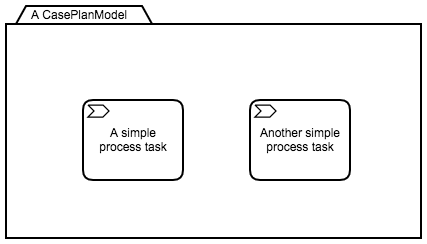
\includegraphics[width=0.7\textwidth]{../figures/chapter_combinations/CMMN_Process_Tasks.png}
      \caption{A CMMN process task to call a BPMN process.}
      \label{fig:CMMN_process_task}
\end{figure}

There are two ways of combination: integrating CMMN in a BPMN model and the opposite way. \\
Figure \ref{fig:CMMN_process_task} illustrates a simple Case Plan Model containing two tasks: \texttt{A simple process task} and \texttt{Another simple process task}. Both "[...] can be used in the Case to call a Business Process" \cite{CMMNspec2014}. As the CMMN specification stated, this is a \textit{call activity} with the intention to direct the process into another (sub-) process. A brief look at the meta model proves this hypothesis by the following attributes of the CMMN process task: \texttt{implementationType : URI}\footnote{Read \texttt{<attribute> : <type>}}, \texttt{inputs : ProcessParameter} and \texttt{outputs : ProcessParameter} \cite{CMMNspec2014}. The \texttt{implementationType} attribute indicates the link to other processes, namely \ac{BPMN}, \ac{XPDL} version 2.x, \ac{WSBPEL} 2.0 and  \ac{WSBPEL} 1.0. The called processes are handed over zero or more input parameters and return the results as output parameters, subsequently processed by the main process. \\
How this link between both models is visually presented depends on the tool the analyst uses. Camunda, for example, uses attributes to link the processes. Signavio links the models directly, so the user only has to click the process symbol in the upper right corner of a process task to switch the models. Though, it is not possible to explicit model BPMN in the CMMN notation, which holds for all notations: BPMN, CMMN and DMN. It is possible to link them, but no to create BPMN models with e.g. the notation set of CMMN. As CMMN is a fairly new specification, the way how combined models can be presented to the user might vary until the tools support the standard completely. \\

\begin{figure}
  \centering
    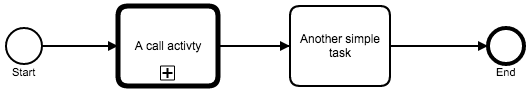
\includegraphics[width=0.7\textwidth]{../figures/chapter_combinations/BPMN_Call_Task.png}
      \caption{A BPMN model with a call activity and an unspecified task.}
      \label{fig:BPMN_call_activity}
\end{figure}

BPMN does not provide any designated interface that links to Case Management or CMMN in particular+, but a workaround is possible similar to the link CMMN to BPMN. \\
In Fig. \ref{fig:BPMN_call_activity} a very small business process is shown, modeled in BPMN. It comprises a \texttt{call activity} and a very simple \texttt{task}. Here, the call activity is able to integrate a CMMN model. According to the BPMN specification, "a call activity identifies a point in the process, where a global process or a global task is used" \cite{BPMNspec}. Again, the meta model proves the ability to link different processes. A Call activity has an attribute \texttt{calledElement: CallableElement} that instantiates an object of the super class \texttt{CallableElement}. This super class provides an \texttt{ioSpecification} and an \texttt{ioBinding} attribute as well as a specification of the used interface. Eventually, the \texttt{ioBinding} allows to define the inputs and outputs as well as one or more operations on the data sets. The \texttt{ioSpecification} is used to specify the inputs and outputs of the activity, whereas the \texttt{ioBinding} becomes necessary when the Call Activity is linked to a service instead of a process \cite{BPMNspec}.
Consequently, a globally defined\footnote{Globally defined means the called object is not a sub-object that can only be instantiated with the main object. Globally defined objects can be called and instatiated.} CMMN case (which can also referred to as a process) can be called here. As the call activity is not a native CMMN-link, the \texttt{CallActivityType} needs to be set to CMMN. Additionally, each call activity has to deliver an output value that is generated during the execution \cite{BPMNspec}. When invoking a process it is necessary to keep in mind that a call activity is able to override the attributes of a called process. Consequently, the behavior of the called process might change \cite{BPMNspec}.\\

In BPMN, a token traverses the model. Each gateway either directs the token to another direction or even multiplies it (AND gateway). At each endpoint of the process model, only one token arrives and ends the instance of the process. By inserting a call activity in BPMN, the token is blocked until the called process ends and escalates the result to the calling process. Consequently, the called process could call another one and this one could also call a process leading to a huge capacity usage and consequently to an abortion of the instance. To avoid this situation, BPMN provides the \texttt{Termination Event} that, when reached by a token, terminates the process immediately and discards the other tokens.

\section{Combining DMN with BPMN}
The "DMN notation is designed to be usable alongside the standard BPMN business process notation" states the first paragraph in the DMN specification \cite{DMNspec2016}. Consequently, DMN serves as a complementary language to BPMN and helps to "[...] create lighter, more focused processes by moving decision details into DMN" \cite{DMNmicroguide}. This leads to a clear structure without a vast amount of gateways and faster processing. Generally speaking, the standalone version of DMN is useful for modeling decisions and their requirements with the \ac{DRG}. The benefits of DMN can be used to a full extent, however, by combining it with another modeling language, for instance BPMN. \\
BPMN has one designated interface for DMN decision logic and several more or less well-suited ones. Table \ref{tab:BPMN_elements_DMN_compatibility} shows BPMN's interface tasks explained by the DMN specification. It stands out that the Business Rule Task is the designated interface, since the BPMN specification defines it as a "[...] mechanism for the Process to provide input to a Business Rules Engine and to get the output of calculations that the Business Rules Engine might provide" \cite{BPMNspec}. As a matter of fact, this is the main purpose of the DMN notation. \\
Figure \ref{fig:DMN_table_in_BusinessRuleTask} illustrates the combination of a BPMN model and the DMN decision logic and how it is implemented by the signavio modeler. The Business Rule Task has an attribute that links to the DMN model and calls the decision with the input parameters. According to the decision logic, the parameter is matched with the correct rule leading to the desired output. In this example, the salary of an employee along with additional privileges needs to be calculated. Obviously, this seems to be a predefined and fully repeatable task combined with a data-centric decision. Although it is possible to model both characteristics in BPMN, it is better to separate them according to their concerns. This leads to simpler models and better performance. \\
The example company employs only three different roles: executives, knowledge workers and routine workers. Each position is paid accordingly and gets an additional privilege. The executive, for instance, gets a salary of 3000 EUR. coupled with a company vehicle. In BPMN, the process sends the parameter to the decision engine and returns the right salary, which is paid after the calculation. The payment procedure is denoted as a script task incorporating the automated payment. According to table \ref{tab:BPMN_elements_DMN_compatibility}, a script task is used for automated decision execution, which can be verified by the example. 

Debevoise and Taylor identified common patterns for the combination of DMN and BPMN in \cite{DMNmicroguide}:
\begin{itemize}
\item \textit{Task Sequencing (inclusive)}: A DMN decision can guide the control flow into one or more subsequent, parallel executed tasks connected by an \texttt{AND}-gateway (also called \textit{inclusive} gateways). 
\item \textit{Participant Assignment}: Responsibilities are usually illustrated by pools and swim lanes. The DMN decision logic can identify the correct swim lane and guide the control flow with an \texttt{XOR}-gateway there.
\item \textit{Effect or Gateway Sequencing (exclusive)}: The same as \textit{Task sequencing} but with \texttt{XOR}-gateways.
\item \textit{Data Information}: DMN is data-centric notation and suits well for data validation and data warehousing. Meta information such as age, origin and accessibility can be managed by DMN tables and stored in the correct database or presented the right person. 
\item \textit{Detection of Events}:  So called \textit{detection decisions} \cite{DMNmicroguide} react to internal or external events. External events are defined as a weather change, security events, or can be issued by customers as well as contractual partners. Internal ones arise from process activities and related steps. An event might eventually make a process adapt to changing circumstances in order to create the same value. Detecting decisions represent the switch that regulate the process accordingly and make it react the occurring events. 
\end{itemize}

So far, only the integration of DMN into a BPMN process model was described. Apparently, integration works seamlessly and complements the BPMN notation. Next, integrating a BPMN model into DMN will be examined. \\
Recapturing the examination of the DMN notation in Chapter \ref{chapter:indicators} recalls the four distinct elements: 
\begin{itemize}
\item the Decision encapsulating the decision logic
\item the Business Knowledge Model which is basically a decision that can be reused and parameterized \cite{DMNmicroguide}
\item the Knowledge Source representing the authoritative foundation 
\item and the Input Data elements that are necessary to make the decision.
\end{itemize}

The only possible interface to integrate another modeling language in DMN could be the Knowledge Source element, as the Business Knowledge Model also encapsulates decision logic. According to the DMN meta model, Knowledge Source elements inherit from \texttt{DRGElement} (similar to an interface class in java) and from \texttt{NamedElement} "[...] from which it inherits [the attributes \texttt{name}, optional \texttt{id}, \texttt{description} and \texttt{label}" \cite{DMNspec2016}. Additionally, the element has three distinct attributes: \texttt{type} of type string, \texttt{owner} of type \texttt{OrganisationalUnit} and the \texttt{locationURI} of type \texttt{URI}. The \texttt{type} attribute is intended to identify the "kind of authoritative source" such as "policies, regulations or analytic insights" \cite{DMNspec2016}. The Uniform Resource Identifier (URI) specifies the concrete location where the authoritative source can be found. \\
In BPMN and CMMN, the interface tasks have designated attributes to call or reference processes. In CMMN, a process task has the attribute \texttt{ProcessRef} of type \texttt{Process} specifically to link different processes \cite{CMMNspec2014}. The BPMN Business Rule Task provides an attribute called \texttt{implementation} that states the technology used to perform the task \cite{BPMNspec}. The DMN meta model, however, lacks these interface tasks and, in particular, the necessary attribute to reference a different process. The Knowledge Source element's \texttt{URI} could link to a process, but it still lacks the \texttt{implementation} attribute that specifies the process type. The \texttt{URI}'s intention is only to provide a specific description where the authoritative documentation can be found.

In conclusion, integrating different models in DMN does not work yet. The current version at the time this thesis was developed was DMN 1.0 from May 2016. As seen in BPMN, it is possible to extend the set of elements of a notation and to make interfaces available. Comprising only four elements, the DMN notation is more a complementing instead of a standalone model as shown in this section. Separating the decision logic in DMN and including them in a BPMN model makes the models easier to model, better to understand and eventually perform faster including run-time adjustment of the decision logic.
% ------------------------------------------------------------------------------------------------------------
% 
% TABLE  ||
%            v
%
\begin{table}[ht]
\centering
\begin{tabular}{*{2}{m{0.48\textwidth}}}
\hline 
Decision Role & Activity Type Role \\
\hline
Apart from looping or multiple instantiating tasks, loops have no decision role. They can help to iterate through decisional steps. &\begin{center}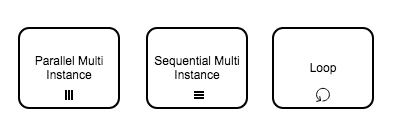
\includegraphics[scale=0.5]{../figures/chapter_combinations/BPMN_Task_Table/Multi_instance.png} \end{center}\\
\hline
A service task executes decisison in an automated way. The corresponding decision model, however, does not guarantee the automated execution. &\begin{center}
\includegraphics[scale=0.7]{../figures/chapter_combinations/BPMN_Task_Table/Service_task.png} \end{center}\\
\hline
The assignee has to execute the decision manually. &\begin{center}\includegraphics[scale=0.7]{../figures/chapter_combinations/BPMN_Task_Table/User_task.png} \end{center}\\
\hline
The Business Rule Task is defined as a placeholder according to \cite{BPMNspec} for decisional services. This is the predefined inteface for DMN models. &\begin{center}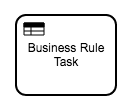
\includegraphics[scale=0.7]{../figures/chapter_combinations/BPMN_Task_Table/Business_rule_task.png} \end{center}\\
\hline
Decisions can be encoded by process scrip languages.  &\begin{center}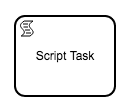
\includegraphics[scale=0.7]{../figures/chapter_combinations/BPMN_Task_Table/Script_task.png} \end{center}\\
\hline
\end{tabular}
\caption{BPMN elements and their DMN compatibility, adopted from Table 70 in \cite{DMNspec2016}.}
\label{tab:BPMN_elements_DMN_compatibility} 
\end{table}
%
%------------------------------------------------------------------------------------------------------------------------
% FIGURE ||
%            v     
%
\begin{figure}
\centering 
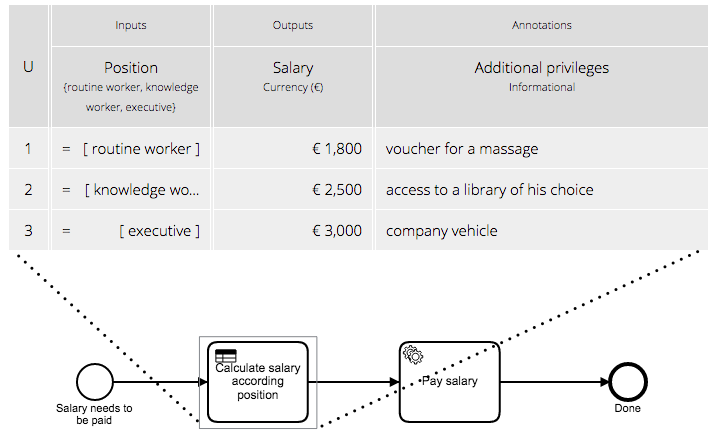
\includegraphics[width=\textwidth]{../figures/chapter_combinations/BPMN_DMN_Salary_2in1.png} 
\caption{The DMN decision logic implemented as a BPMN business rule (illustrating example).}
\label{fig:DMN_table_in_BusinessRuleTask}
\end{figure}
%
%--------------------------------------------------------------------------------------------------------------------------------------------;;;;;;;;;;;;;;;;;;;;;;;;;;;;;;;;;;;;;;;;;;;;;;;;;;;;;;;;;;;;;;;;;;;;;;;;;;;;;;;;;;;;;;;;;;;;;;;;;;;;;;;;;;;;;;;;;;;;;;;;;;;;;;;;;;;;;;;;;;;;;;;;;;;;;;;;;;;;;;;;;;;;;;;;;;;;;;;;;;;;;;;;;;;;;;;;;;;;;;;;;;;;;;;;;;;;;;;;;;;;;;;;;;;;;;;;;;;;;;;;;;;;;;;;;;;;;;;;;;;;;;;;;;;;;;;;;;;;;;;;;;;;;;;;;;;;;;;;;;;;;;;;;;;;;;;;;;;;;;;;;;;;;;;;;;;;;;;;;;;;;;;;;;;;;;;;;;;;;;;;;;;;;;;;;;;;;;;;;;;;;;;;;;;;;;;;;;;;;;;;;;;;;;;;;;;;;;;;;;;;;;;;;;;;;;;;;;;;;;;;;;;;;;;;;;;;;;;;;;;;;;;;;;;;;;;;;;;;;;;;;;;;;;;;;;;;;;;;;;;;;;;;;;;;;;;;;;;;;;;;;;;;;;;;;;;;;;;;;;;;;;;;;;;;;;;;;;;;;;;;;;;;;;;;;;;;;;;;;;;;;;;;;;;;;;;;;;;;;;;;;;;;;;;;;;;;;;;;;;;;;;;;;;;;;;;;;;;;;;;;;;;;;;;;;;;;;;;;;;;;;;;;;;;;;;;;;;;;;;;;;;;;;;;;;;;;;;;;;;;;;;;;;;;;;;;;;;;;;;;;;;;;;;;;;;;;;;;;;;;;;;;;;;;;;;;;;;;;;;;;;;;;;;;;;;;;;;;;;;;;;;;;;;;;;;;;;;;;;;;;;;;;;;;;;;;;;;;;;;;;;;;;;;;;;;;;;;;;;;;;;;;;;;;;;;;;;;;;;;;;;;;;;;;;;;;;;;;;;;;;;;;;;;;;;;;;;;;;;;;;;;;;;;;;;;;;;;;;;;;;;;;;;;;;;;;;;;;;;;;;;;;;;;;;;;;;;;;;;;;;;;;;;;;;;;;;;;;;;;;;;;;;;;;;;;;;;;;;;;;;;;;;;;;;;;;;;;;;;;;;;;;;;;;;;;;;;;;;;;;;;;;;;;;;;;;;;;;;;;;;;;;;;;;;;;;;;;;;;;;;;;;;;;;;;;;;;;;;;;;;;;;;;;;;;;;;;;;;;;;;;;;;;;;;;;;;;;;;;;;;;;;;;;;;;;;;;;;;;;;;;;;;;;;;;;;;;;;;;;;;;;;;;;;;;;;;;;;;;;;;;;;;;;;;;;;;;;;;;;;;;;;;;;;;;;;;;;;;;;;;;;;;;;;;;;;;;;;;;;;;;;;;;;;;;;;;;;;;;;;;;;;;;;;;;;;;;;;;;;;;;;;;;;;;;;;;;;;;;;;;;;;;;;;;;;;;;;;;;;;;;;;;;;;;;;;;;;;;;;;;;;;;;;;;;;;;;;;;;;;;;;;;;;;;;;;;;;;;;;;;;;;;;;;;;;;;;;;;;;;;;;;;;;;;;;;;;;;;;;;;;;;;;;;;;;;;;;;;;;;;;;;;;;;;;;;;;;;;;;;;;;;;;;;;;;;;;;;;;;;;;;;;;;;;;;;;;;;;;;;;;;;;;;;;;;;;;;;;;;;;;;;;;;;;;;;;;;;;;;;;;;;;;;;;;;;;;;;;;;;;;;;;;;;;;;;;;;;;;;;;;;;;;;;;;;;;;;;;;;;;;;;;;;;;;;;;;;;;;;;;;;;;;;;;;;;;;;;;;;;;;;;;;;;;;;;;;;;;;;;;;;;;;;;;;;;;;;;;;;;;;;;;;;;;;;;;;;;;;;;;;;;;;;;;;;;;;;;;;;;;;;;;;;;;;;;;;;;;;;;;;;;;;;;;;;;;;;;;;;;;;;;;;;;;;;;;;;;;;;;;;;;;;;;;;;;;;;;;;;;;;;;;;;;;;;;;;;;;;;;;;;;;;;;;;;;;;;;;;;;;;;;;;;;;;;;;;;;;;;;;;;;;;;;;;;;;;;;;;;;;;;;;;;;;;;;;;;;;;;;;;;;;;;;;;;;;;;;;;;;;;;;;;;;;;;;;;;;;;;;;;;;;;;;;;;;;;;;;;;;;;;;;;;;;;;;;;;;;;;;;;;;;;;;;;;;;;;;;;;;;;;;;;;;;;;;;;;;;;;;;;;;;;;;;;;;;;;;;;;;;;;;;;;;;;;;;;;;;;;;;;;;;;;;;;;;;;;;;;;;;;;;;;;;;;;;;;;;;;;;;;;;;;;;;;;;;;;;;;;;;;;;;;;;;;;;;;;;;;;;;;;;;;;;;;;;;;;;;;;;;;;;;;;;;;;;;;;;;;;;;;;;;;;;;;;;;;;;;;;;;;;;;;;;;;;;;;;;;;;;;;;;;;;;;;;;;;;;;;;;;;;;;;;;;;;;;;;;;;;;;;;;;;;;;;;;;;;;;;;;;;;;;;;;;;;;;;;;;;;;;;;;;;;;;;;;;;;;;;;;;;;;;;;;;;;;;;;;;;;;;;;;;;;;;;;;;;;;;;;;;;;;;;;;;;;;;;;;;;;;;;;;;;;;;;;;;;;;;;;;;;;;;;;;;;;;;;;;;;;;;;;;;;;;;;;;;;;;;;;;;;;;;;;;;;;;;;;;;;;;;;;;;;;;;;;;;;;;;;;;;;;;;;;;;;;;;;;;;;;;;;;;;;;;;;;;;;;;;;;;;;;;;;;;;;;;;;;;;;;;;;;;;;;;;;;;;;;;;;;;;;;;;;;;;;;;;;;;;;;;;;;;;;;;;;;;;;;;;;;;;;;;;;;;;;;;;;;;;;;;;;;;;;;;;;;;;;;;;;;;;;;;;;;;;;;;;;;;;;;;;;;;;;;;;;;;;;;;;;;;;;;;;;;;;;;;;;;;;;;;;;;;;;;;;;;;;;;;;;;;;;;;;;;;;;;;;;;;;;;;;;;;;;;;;;;;;;;;;;;;;;;;;;;;;;;;;;;;;;;;;;;;;;;;;;;;;;;;;;;;;;;;;;;;;;;;;;;;;;;;;;;;;;;;;;;;;;;;;;;;;;;;;;;;;;;;;;;;;;;;;;;;;;;;;;;;;;;;;;;;;;;;;;;;;;;;;;;;;;;;;;;;;;;;;;;;;;;;;;;;;;;;;;;;;;;;;;;;;;;;;;;;;;;;;;;;;;;;;;;;;;;;;;;;;;;;;;;;;;;;;;;;;;;;;;;;;;;;;;;;;;;;;;;;;;;;;;;;;;;;;;;;;;;;;;;;;;;;;;;;;;;;;;;;;;;;;;;;;;;;;;;;;;;;;;;;;;;;;;;;;;;;;;;;;;;;;;;;;;;;;;;;;;;;;;;;;;;;;;;;;;;;;;;;;;;;;;;;;;;;;;;;;;;;;;;;;;;;;;;;;;;;;;;;;;;;;;;;;;;;;;;;;;;;;;;;;;;;;;;;;;;;;;;;;;;;;;;;;;;;;;;;;;;;;;;;;;;;;;;;;;;;;;;;;;;;;;;;;;;;;;;;;;;;;;;;;;;;;;;;;;;;;;;;;;;;;;;;;;;;;;;;;;;;;;;;;;;;;;;;;;;;;;;;;;;;;;;;;;;;;;;;;;;;;;;;;;;;;;;;;;;;;;;;;;;;;;;;;;;;;;;;;;;;;;;;;;;;;;;;;;;;;;;;;;;;;;;;;;;;;;;;;;;;;;;;;;;;;;;;;;;;;;;;;;;;;;;;;;;;;;;;;;;;;;;;;;;;;;;;;;;;;;;;;;;;;;;;;;;;;;;;;;;;;;;;;;;;;;;;;;;;;;;;;;;;;;;;;;;;;;;;;;;;;;;;;;;;;;;;;;;;;;;;;;;;;;;;;;;;;;;;;;;;;;;;;;;;;;;;;;;;;;;;;;;;;;;;;;;;;;;;;;;;;;;;;;;;;;;;;;;;;;;;;;;;;;;;;;;;;;;;;;;;;;;;;;;;;;;;;;;;;;;;;;;;;;;;;;;;;;;;;;;;;;;;;;;;;;;;;;;;;;;;;;;;;;;;;;;;;;;;;;;;;;;;;;;;;;;;;;;;;;;;;;;;;;;;;;;;;;;;;;;;;;;;;;;;;;;;;;;;;;;;;;;;;;;;;;;;;;;;;;;;;;;;;;;;;;;;;;;;;;;;;;;;;;;;;;;;;;;;;;;;;;;;;;;;;;;;;;;;;;;;;;;;;;;;;;;;;;;;;;;;;;;;;;;;;;;;;;;;;;;;;;;;;;;;;;;;;;;;;;;;;;;;;;;;;;;;;;;;;;;;;;;;;;;;;;;;;;;;;;;;;;;;;;;;;;;;;;;;;;;;;;;;;;;;;;;;;;;;;;;;;;;;;;;;;;;;;;;;;;;;;;;;;;;;;;;;;;;;;;;;;;;;;;;;;;;;;;;;;;;;;;;;;;;;;;;;;;;;;;;;;;;;;;;;;;;;;;;;;;;;;;;;;;;;;;;;;;;;;;;;;;;;;;;;;;;;;;;;;;;;;;;;;;;;;;;;;;;;;;;;;;;;;;;;;;;;;;;;;;;;;;;;;;;;;;;;;;;;;;;;;;;;;;;;;;;;;;;;;;;;;;;;;;;;;;;;;;;;;;;;;;;;;;;;;;;;;;;;;;;;;;;;;;;;;;;;;;;;;;;;;;;;;;;;;;;;;;;;;;;;;;;;;;;;;;;;;;;;;;;;;;;;;;;;;;;;;;;;;;;;;;;;;;;;;;;;;;;;;;;;;;;;;;;;;;;;;;;;;;;;;;;;;;;;;;;;;;;;;;;;;;;;;;;;;;;;;;;;;;;;;;;;;;;;;;;;;;;;;;;;;;;;;;;;;;;;;;;;;;;;;;;;;;;;;;;;;;;;;;;;;;;;;;;;;;;;;;;;;;;;;;;;;;;;;;;;;;;;;;;;;;;;;;;;;;;;;;;;;;;;;;;;;;;;;;;;;;;;;;;;;;;;;;;;;;;;;;;;;;;;;;;;;;;;;;;;;;;;;;;;;;;;;;;;;;;;;;;;;;;;;;;;;;;;;;;;;;;;;;;;;;;;;;;;;;;;;;;;;;;;;;;;;;;;;;;;;;;;;;;;;;;;;;;;;;;;;;;;;;;;;;;;;;;;;;;;;;;;;;;;;;;;;;;;;;;;;;;;;;;;;;;;;;;;;;;;;;;;;;;;;;;;;;;;;;;;;;;;;;;;;;;;;;;;;;;;;;;;;;;;;;;;;;;;;;;;;;;;;;;;;;;;;;;;;;;;;;;;;;;;;;;;;;;;;;;;;;;;;;;;;;;;;;;;;;;;;;;;;;;;;;;;;;;;;;;;;;;;;;;;;;;;;;;;;;;;;;;;;;;;;;;;;;;;;;;;;;;;;;;;;;;;;;;;;;;;;;;;;;;;;;;;;;;;;;;;;;;;;;;;;;;;;;;;;;;;;;;;;;;;;;;;;;;;;;;;;;;;;;;;;;;;;;;;;;;;;;;;;;;;;;;;;;;;;;;;;;;;;;;;;;;;;;;;;;;;;;;;;;;;;;;;;;;;;;;;;;;;;;;;;;;;;;;;;;;;;;;;;;;;;;;;;;;;;;;;;;;;;;;;;;;;;;;;;;;;;;;;;;;;;;;;;;;;;;;;;;;;;;;;;;;;;;;;;;;;;;;;;;;;;;;;;;;;;;;;;;;;;;;;;;;;;;;;;;;;;;;;;;;;;;;;;;;;;;;;;;;;;;;;;;;;;;;;;;;;;;;;;;;;;;;;;;;;;;;;;;;;;;;;;;;;;;;;;;;;;;;;;;;;;;;;;;;;;;;;;;;;;;;;;;;;;;;;;;;;;;;;;;;;;;;;;;;;;;;;;;;;;;;;;;;;;;;;;;;;;;;;;;;;;;;;;;;;;;;;;;;;;;;;;;;;;;;;;;;;;;;;;;;;;;;;;;;;;;;;;;;;;;;;;;;;;;;;;;;;;;;;;;;;;;;;;;;;;;;;;;;;;;;;;;;;;;;;;;;;;;;;;;;;;;;;;;;;;;;;;;;;;;;;;;;;;;;;;;;;;;;;;;;;;;;;;;;;;;;;;;;;;;;;;;;;;;;;;;;;;;;;;;;;;;;;;;;;;;;;;;;;;;;;;;;;;;;;;;;;;;;;;;;;;;;;;;;;;;;;;;;;;;;;;;;;;;;;;;;;;;;;;;;;;;;;;;;;;;;;;;;;;;;;;;;;;;;;;;;;;;;;;;;;;;;;;;;;;;;;;;;;;;;;;;;;;;;;;;;;;;;;;;;;;;;;;;;;;;;;;;;;;;;;;;;;;;;;;;;;;;;;;;;;;;;;;;;;;;;;;;;;;;;;;;;;;;;;;;;;;;;;;;;;;;;;;;;;;;;;;;;;;;;;;;;;;;;;;;;;;;;;;;;;;;;;;;;;;;;;;;;;;;;;;;;;;;;;;;;;;;;;;;;;;;;;;;;;;;;;;;;;;;;;;;;;;;;;;;;;;;;;;;;;;;;;;;;;;;;;;;;;;;;;;;;;;;;;;;;;;;;;;;;;;;;;;;;;;;;;;;;;;;;;;;;;;;;;;;;;;;;;;;;;;;;;;;;;;;;;;;;;;;;;;;;;;;;;;;;;;;;;;;;;;;;;;;;;;;;;;;;;;;;;;;;;;;;;;;;;;;;;;;;;;;;;;;;;;;;;;;;;;;;;;;;;;;;;;;;;;;;;;;;;;;;;;;;;;;;;;;;;;;;;;;;;;;;;;;;;;;;;;;;;;;;;;;;;;;;;;;;;;;;;;;;;;;;;;;;;;;;;;;;;;;;;;;;;;;;;;;;;;;;;;;;;;;;;;;;;;;;;;;;;;;;;;;;;;;;;;;;;;;;;;;;;;;;;;;;;;;;;;;;;;;;;;;;;;;;;;;;;;;;;;;;;;;;;;;;;;;;;;;;;;;;;;;;;;;;;;;;;;;;;;;;;;;;;;;;;;;;;;;;;;;;;;;;;;;;;;;;;;;;;;;;;;;;;;;;;;;;;;;;;;;;;;;;;;;;;;;;;;;;;;;;;;;;;;;;;;;;;;;;;;;;;;;;;;;;;;;;;;;;;;;;;;;;;;;;;;;;;;;;;;;;;;;;;;;;;;;;;;;;;;;;;;;;;;;;;;;;;;;;;;;;;;;;;;;;;;;;;;;;;;;;;;;;;;;;;;;;;;;;;;;;;;;;;;;;;;;;;;;;;;;;;;;;;;;;;;;;;;;;;;;;;;;;;;;;;;;;;;;;;;;;;;;;;;;;;;;;;;;;;;;;;;;;;;;;;;;;;;;;;;;;;;;;;;;;;;;;;;;;;;;;;;;;;;;;;;;;;;;;;;;;;;;;;;;;;;;;;;;;;;;;;;;;;;;;;;;;;;;;;;;;;;;;;;;;;;;;;;;;;;;;;;;;;;;;;;;;;;;;;;;;;;;;;;;;;;;;;;;;;;;;;;;;;;;;;;;;;;;;;;;;;;;;;;;;;;;;;;;;;;;;;;;;;;;;;;;;;;;;;;;;;;;;;;;;;;;;;;;;;;;;;;;;;;;;;;;;;;;;;;;;;;;;;;;;;;;;;;;;;;;;;;;;;;;;;;;;;;;;;;;;;;;;;;;;;;;;;;;;;;;;;;;;;;;;;;;;;;;;;;;;;;;;;;;;;;;;;;;;;;;;;;;;;;;;;;;;;;;;;;;;;;;;;;;;;;;;;;;;;;;;;;;;;;;;;;;;;;;;;;;;;;;;;;;;;;;;;;;;;;;;;;;;;;;;;;;;;;;;;;;;;;;;;;;;;;;;;;;;;;;;;;;;;;;;;;;;;;;;;;;;;;;;;;;;;;;;;;;;;;;;;;;;;;;;;;;;;;;;;;;;;;;;;;;;;;;;;;;;;;;;;;;;;;;;;;;;;;;;;;;;;;;;;;;;;;;;;;;;;;;;;;;;;;;;;;;;;;;;;;;;;;;;;;;;;;;;;;;;;;;;;;;;;;;;;;;;;;;;;;;;;;;;;;;;;;;;;;;;;;;;;;;;;;;;;;;;;;;;;;;;;;;;;;;;;;;;;;;;;;;;;;;;;;;;;;;;;;;;;;;;;;;;;;;;;;;;;;;;;;;;;;;;;;;;;;;;;;;;;;;;;;;;;;;;;;;;;;;;;;;;;;;;;;;;;;;;;;;;;;;;;;;;;;;;;;;;;;;;;;;;;;;;;;;;;;;;;;;;;;;;;;;;;;;;;;;;;;;;;;;;;;;;;;;;;;;;;;;;;;;;;;;;;;;;;;;;;;;;;;;;;;;;;;;;;;;;;;;;;;;;;;;;;;;;;;;;;;;;;;;;;;;;;;;;;;;;;;;;;;;;;;;;;;;;;;;;;;;;;;;;;;;;;;;;;;;;;;;;;;;;;;;;;;;;;;;;;;;;;;;;;;;;;;;;;;;;;;;;;;;;;;;;;;;;;;;;;;;;;;;;;;;;;;;;;;;;;;;;;;;;;;;;;;;;;;;;;;;;;;;;;;;;;;;;;;;;;;;;;;;;;;;;;;;;;;;;;;;;;;;;;;;;;;;;;;;;;;;;;;;;;;;;;;;;;;;;;;;;;;;;;;;;;;;;;;;;;;;;;;;;;;;;;;;;;;;;;;;;;;;;;;;;;;;;;;;;;;;;;;;;;;;;;;;;;;;;;;;;;;;;;;;;;;;;;;;;;;;;;;;;;;;;;;;;;;;;;;;;;;;;;;;;;;;;;;;;;;;;;;;;;;;;;;;;;;;;;;;;;;;;;;;;;;;;;;;;;;;;;;;;;;;;;;;;;;;;;;;;;;;;;;;;;;;;;;;;;;;;;;;;;;;;;;;;;;;;;;;;;;;;;;;;;;;;;;;;;;;;;;;;;;;;;;;;;;;;;;;;;;;;;;;;;;;;;;;;;;;;;;;;;;;;;;;;;;;;;;;;;;;;;;;;;;;;;;;;;;;;;;;;;;;;;;;;;;;;;;;;;;;;;;;;;;;;;;;;;;;;;;;;;;;;;;;;;;;;;;;;;;;;;;;;;;;;;;;;;;;;;;;;;;;;;;;;;;;;;;;;;;;;;;;;;;;;;;;;;;;;;;;;;;;;;;;;;;;;;;;;;;;;;;;;;;;;;;;;;;;;;;;;;;;;;;;;;;;;;;;;;;;;;;;;;;;;;;;;;;;;;;;;;;;;;;;;;;;;;;;;;;;;;;;;;;;;;;;;;;;;;;;;;;;;;;;;;;;;;;;;;;;;;;;;;;;;;;;;;;;;;;;;;;;;;;;;;;;;;;;;;;;;;;;;;;;;;;;;;;;;;;;;;;;;;;;;;;;;;;;;;;;;;;;;;;;;;;;;;;;;;;;;;;;;;;;;;;;;;;;;;;;;;;;;;;;;;;;;;;;;;;;;;;;;;;;;;;;;;;;;;;;;;;;;;;;;;;;;;;;;;;;;;;;;;;;;;;;;;;;;;;;;;;;;;;;;;;;;;;;;;;;;;;;;;;;;;;;;;;;;;;;;;;;;;;;;;;;;;;;;;;;;;;;;;;;;;;;;;;;;;;;;;;;;;;;;;;;;;;;;;;;;;;;;;;;;;;;;;;;;;;;;;;;;;;;;;;;;;;;;;;;;;;;;;;;;;;;;;;;;;;;;;;;;;;;;;;;;;;;;;;;;;;;;;;;;;;;;;;;;;;;;;;;;;;;;;;;;;;;;;;;;;;;;;;;;;;;;;;;;;;;;;;;;;;;;;;;;;;;;;;;;;;;;;;;;;;;;;;;;;;;;;;;;;;;;;;;;;;;;;;;;;;;;;;;;;;;;;;;;;;;;;;;;;;;;;;;;;;;;;;;;;;;;;;;;;;;;;;;;;;;;;;;;;;;;;;;;;;;;;;;;;;;;;;;;;;;;;;;;;;;;;;;;;;;;;;;;;;;;;;;;;;;;;;;;;;;;;;;;;;;;;;;;;;;;;;;;;;;;;;;;;;;;;;;;;;;;;;;;;;;;;;;;;;;;;;;;;;;;;;;;;;;;;;;;;;;;;;;;;;;;;;;;;;;;;;;;;;;;;;;;;;;;;;;;;;;;;;;;;;;;;;;;;;;;;;;;;;;;;;;;;;;;;;;;;;;;;;;;;;;;;;;;;;;;;;;;;;;;;;;;;;;;;;;;;;;;;;;;;;;;;;;;;;;;;;;;;;;;;;;;;;;;;;;;;;;;;;;;;;;;;;;;;;;;;;;;;;;;;;;;;;;;;;;;;;;;;;;;;;;;;;;;;;;;;;;;;;;;;;;;;;;;;;;;;;;;;;;;;;;;;;;;;;;;;;;;;;;;;;;;;;;;;;;;;;;;;;;;;;;;;;;;;;;;;;;;;;;;;;;;;;;;;;;;;;;;;;;;;;;;;;;;;;;;;;;;;;;;;;;;;;;;;;;;;;;;;;;;;;;;;;;;;;;;;;;;;;;;;;;;;;;;;;;;;;;;;;;;;;;;;;;;;;;;;;;;;;;;;;;;;;;;;;;;;;;;;;;;;;;;;;;;;;;;;;;;;;;;;;;;;;;;;;;;;;;;;;;;;;;;;;;;;;;;;;;;;;;;;;;;;;;;;;;;;;;;;;;;;;;;;;;;;;;;;;;;;;;;;;;;;;;;;;;;;;;;;;;;;;;;;;;;;;;;;;;;;;;;;;;;;;;;;;;;;;;;;;;;;;;;;;;;;;;;;;;;;;;;;;;;;;;;;;;;;;;;;;;;;;;;;;;;;;;;;;;;;;;;;;;;;;;;;;;;;;;;;;;;;;;;;;;;;;;;;;;;;;;;;;;;;;;;;;;;;;;;;;;;;;;;;;;;;;;;;;;;;;;;;;;;;;;;;;;;;;;;;;;;;;;;;;;;;;;;;;;;;;;;;;;;;;;;;;;;;;;;;;;;;;;;;;;;;;;;;;;;;;;;;;;;;;;;;;;;;;;;;;;;;;;;;;;;;;;;;;;;;;;;;;;;;;;;;;;;;;;;;;;;;;;;;;;;;;;;;;;;;;;;;;;;;;;;;;;;;;;;;;;;;;;;;;;;;;;;;;;;;;;;;;;;;;;;;;;;;;;;;;;;;;;;;;;;;;;;;;;;;;;;;;;;;;;;;;;;;;;;;;;;;;;;;;;;;;;;;;;;;;;;;;;;;;;;;;;;;;;;;;;;;;;;;;;;;;;;;;;;;;;;;;;;;;;;;;;;;;;;;;;;;;;;;;;;;;;;;;;;;;;;;;;;;;;;;;;;;;;;;;;;;;;;;;;;;;;;;;;;;;;;;;;;;;;;;;;;;;;;;;;;;;;;;;;;;;;;;;;;;;;;;;;;;;;;;;;;;;;;;;;;;;;;;;;;;;;;;;;;;;;;;;;;;;;;;;;;;;;;;;;;;;;;;;;;;;;;;;;;;;;;;;;;;;;;;;;;;;;;;;;;;;;;;;;;;;;;;;;;;;;;;;;;;;;;;;;;;;;;;;;;;;;;;;;;;;;;;;;;;;;;;;;;;;;;;;;;;;;;;;;;;;;;;;;;;;;;;;;;;;;;;;;;;;;;;;;;;;;;;;;;;;;;;;;;;;;;;;;;;;;;;;;;;;;;;;;;;;;;;;;;;;;;;;;;;;;;;;;;;;;;;;;;;;;;;;;;;;;;;;;;;;;;;;;;;;;;;;;;;;;;;;;;;;;;;;;;;;;;;;;;;;;;;;;;;;;;;;;;;;;;;;;;;;;;;;;;;;;;;;;;;;;;;;;;;;;;;;;;;;;;;;;;;;;;;;;;;;;;;;;;;;;;;;;;;;;;;;;;;;;;;;;;;;;;;;;;;;;;;;;;;;;;;;;;;;;;;;;;;;;;;;;;;;;;;;;;;;;;;;;;;;;;;;;;;;;;;;;;;;;;;;;;;;;;;;;;;;;;;;;;;;;;;;;;;;;;;;;;;;;;;;;;;;;;;;;;;;;;;;;;;;;;;;;;;;;;;;;;;;;;;;;;;;;;;;;;;;;;;;;;;;;;;;;;;;;;;;;;;;;;;;;;;;;;;;;;;;;;;;;;;;;;;;;;;;;;;;;;;;;;;;;;;;;;;;;;;;;;;;;;;;;;;;;;;;;;;;;;;;;;;;;;;;;;;;;;;;;;;;;;;;;;;;;;;;;;;;;;;;;;;;;;;;;;;;;;;;;;;;;;;;;;;;;;;;;;;;;;;;;;;;;;;;;;;;;;;;;;;;;;;;;;;;;;;;;;;;;;;;;;;;;;;;;;;;;;;;;;;;;;;;;;;;;;;;;;;;;;;;;;;;;;;;;;;;;;;;;;;;;;;;;;;;;;;;;;;;;;;;;;;;;;;;;;;;;;;;;;;;;;;;;;;;;;;;;;;;;;;;;;;;;;;;;;;;;;;;;;;;;;;;;;;;;;;;;;;;;;;;;;;;;;;;;;;;;;;;;;;;;;;;;;;;;;;;;;;;;;;;;;;;;;;;;;;;;;;;;;;;;;;;;;;;;;;;;;;;;;;;;;;;;;;;;;;;;;;;;;;;;;;;;;;;;;;;;;;;;;;;;;;;;;;;;;;;;;;;;;;;;;;;;;;;;;;;;;;;;;;;;;;;;;;;;;;;;;;;;;;;;;;;;;;;;;;;;;;;;;;;;;;;;;;;;;;;;;;;;;;;;;;;;;;;;;;;;;;;;;;;;;;;;;;;;;;;;;;;;;;;;;;;;;;;;;;;;;;;;;;;;;;;;;;;;;;;;;;;;;;;;;;;;;;;;;;;;;;;;;;;;;;;;;;;;;;;;;;;;;;;;;;;;;;;;;;;;;;;;;;;;;;;;;;;;;;;;;;;;;;;;;;;;;;;;;;;;;;;;;;;;;;;;;;;;;;;;;;;;;;;;;;;;;;;;;;;;;;;;;;;;;;;;;;;;;;;;;;;;;;;;;;;;;;;;;;;;;;;;;;;;;;;;;;;;;;;;;;;;;;;;;;;;;;;;;;;;;;;;;;;;;;;;;;;;;;;;;;;;;;;;;;;;;;;;;;;;;;;;;;;;;;;;;;;;;;;;;;;;;;;;;;;;;;;;;;;;;;;;;;;;;;;;;;;;;;;;;;;;;;;;;;;;;;;;;;;;;;;;;;;;;;;;;;;;;;;;;;;;;;;;;;;;;;;;;;;;;;;;;;;;;;;;;;;;;;;;;;;;;;;;;;;;;;;;;;;;;;;;;;;;;;;;;;;;;;;;;;;;;;;;;;;;;;;;;;;;;;;;;;;;;;;;;;;;;;;;;;;;;;;;;;;;;;;;;;;;;;;;;;;;;;;;;;;;;;;;;;;;;;;;;;;;;;;;;;;;;;;;;;;;;;;;;;;;;;;;;;;;;;;;;;;;;;;;;;;;;;;;;;;;;;;;;;;;;;;;;;;;;;;;;;;;;;;;;;;;;;;;;;;;;;;;;;;;;;;;;;;;;;;;;;;;;;;;;;;;;;;;;;;;;;;;;;;;;;;;;;;;;;;;;;;;;;;;;;;;;;;;;;;;;;;;;;;;;;;;;;;;;;;;;;;;;;;;;;;;;;;;;;;;;;;;;;;;;;;;;;;;;;;;;;;;;;;;;;;;;;;;;;;;;;;;;;;;;;;;;;;;;;;;;;;;;;;;;;;;;;;;;;;;;;;;;;;;;;;;;;;;;;;;;;;;;;;;;;;;;;;;;;;;;;;;;;;;;;;;;;;;;;;;;;;;;;;;;;;;;;;;;;;;;;;;;;;;;;;;;;;;;;;;;;;;;;;;;;;;;;;;;;;;;;;;;;;;;;;;;;;;;;;;;;;;;;;;;;;;;;;;;;;;;;;;;;;;;;;;;;;;;;;;;;;;;;;;;;;;;;;;;;;;;;;;;;;;;;;;;;;;;;;;;;;;;;;;;;;;;;;;;;;;;;;;;;;;;;;;;;;;;;;;;;;;;;;;;;;;;;;;;;;;;;;;;;;;;;;;;;;;;;;;;;;;;;;;;;;;;;;;;;;;;;;;;;;;;;;;;;;;;;;;;;;;;;;;;;;;;;;;;;;;;;;;;;;;;;;;;;;;;;;;;;;;;;;;;;;;;;;;;;;;;;;;;;;;;;;;;;;;;;;;;;;;;;;;;;;;;;;;;;;;;;;;;;;;;;;;;;;;;;;;;;;;;;;;;;;;;;;;;;;;;;;;;;;;;;;;;;;;;;;;;;;;;;;;;;;;;;;;;;;;;;;;;;;;;;;;;;;;;;;;;;;;;;;;;;;;;;;;;;;;;;;;;;;;;;;;;;;;;;;;;;;;;;;;;;;;;;;;;;;;;;;;;;;;;;;;;;;;;;;;;;;;;;;;;;;;;;;;;;;;;;;;;;;;;;;;;;;;;;;;;;;;;;;;;;;;;;;;;;;;;;;;;;;;;;;;;;;;;;;;;;;;;;;;;;;;;;;;;;;;;;;;;;;;;;;;;;;;;;;;;;;;;;;;;;;;;;;;;;;;;;;;;;;;;;;;;;;;;;;;;;;;;;;;;;;;;;;;;;;;;;;;;;;;;;;;;;;;;;;;;;;;;;;;;;;;;;;;;;;;;;;;;;;;;;;;;;;;;;;;;;;;;;;;;;;;;;;;;;;;;;;;;;;;;;;;;;;;;;;;;;;;;;;;;;;;;;;;;;;;;;;;;;;;;;;;;;;;;;;;;;;;;;;;;;;;;;;;;;;;;;;;;;;;;;;;;;;;;;;;;;;;;;;;;;;;;;;;;;;;;;;;;;;;;;;;;;;;;;;;;;;;;;;;;;;;;;;;;;;;;;;;;;;;;;;;;;;;;;;;;;;;;;;;;;;;;;;;;;;;;;;;;;;;;;;;;;;;;;;;;;;;;;;;;;;;;;;;;;;;;;;;;;;;;;;;;;;;;;;;;;;;;;;;;;;;;;;;;;;;;;;;;;;;;;;;;;;;;;;;;;;;;;;;;;;;;;;;;;;;;;;;;;;;;;;;;;;;;;;;;;;;;;;;;;;;;;;;;;;;;;;;;;;;;;;;;;;;;;;;;;;;;;;;;;;;;;;;;;;;;;;;;;;;;;;;;;;;;;;;;;;;;;;;;;;;;;;;;;;;;;;;;;;;;;;;;;;;;;;;;;;;;;;;;;;;;;;;;;;;;;;;;;;;;;;;;;;;;;;;;;;;;;;;;;;;;;;;;;;;;;;;;;;;;;;;;;;;;;;;;;;;;;;;;;;;;;;;;;;;;;;;;;;;;;;;;;;;;;;;;;;;;;;;;;;;;;;;;;;;;;;;;;;;;;;;;;;;;;;;;;;;;;;;;;;;;;;;;;;;;;;;;;;;;;;;;;;;;;;;;;;;;;;;;;;;;;;;;;;;;;;;;;;;;;;;;;;;;;;;;;;;;;;;;;;;;;;;;;;;;;;;;;;;;;;;;;;;;;;;;;;;;;;;;;;;;;;;;;;;;;;;;;;;;;;;;;;;;;;;;;;;;;;;;;;;;;;;;;;;;;;;;;;;;;;;;;;;;;;;;;;;;;;;;;;;;;;;;;;;;;;;;;;;;;;;;;;;;;;;;;;;;;;;;;;;;;;;;;;;;;;;;;;;;;;;;;;;;;;;;;;;;;;;;;;;;;;;;;;;;;;;;;;;;;;;;;;;;;;;;;;;;;;;;;;;;;;;;;;;;;;;;;;;;;;;;;;;;;;;;;;;;;;;;;;;;;;;;;;;;;;;;;;;;;;;;;;;;;;;;;;;;;;;;;;;;;;;;;;;;;;;;;;;;;;;;;;;;;;;;;;;;;;;;;;;;;;;;;;;;;;;;;;;;;;;;;;;;;;;;;;;;;;;;;;;;;;;;;;;;;;;;;;;;;;;;;;;;;;;;;;;;;;;;;;;;;;;;;;;;;;;;;;;;;;;;;;;;;;;;;;;;;;;;;;;;;;;;;;;;;;;;;;;;;;;;;;;;;;;;;;;;;;;;;;;;;;;;;;;;;;;;;;;;;;;;;;;;;;;;;;;;;;;;;;;;;;;;;;;;;;;;;;;;;;;;;;;;;;;;;;;;;;;;;;;;;;;;;;;;;;;;;;;;;;;;;;;;;;;;;;;;;;;;;;;;;;;;;;;;;;;;;;;;;;;;;;;;;;;;;;;;;;;;;;;;;;;;;;;;;;;;;;;;;;;;;;;;;;;;;;;;;;;;;;;;;;;;;;;;;;;;;;;;;;;;;;;;;;;;;;;;;;;;;;;;;;;;;;;;;;;;;;;;;;;;;;;;;;;;;;;;;;;;;;;;;;;;;;;;;;;;;;;;;;;;;;;;;;;;;;;;;;;;;;;;;;;;;;;;;;;;;;;;;;;;;;;;;;;;;;;;;;;;;;;;;;;;;;;;;;;;;;;;;;;;;;;;;;;;;;;;;;;;;;;;;;;;;;;;;;;;;;;;;;;;;;;;;;;;;;;;;;;;;;;;;;;;;;;;;;;;;;;;;;;;;;;;;;;;;;;;;;;;;;;;;;;;;;;;;;;;;;;;;;;;;;;;;;;;;;;;;;;;;;;;;;;;;;;;;;;;;;;;;;;;;;;;;;;;;;;;;;;;;;;;;;;;;;;;;;;;;;;;;;;;;;;;;;;;;;;;;;;;;;;;;;;;;;;;;;;;;;;;;;;;;;;;;;;;;;;;;;;;;;;;;;;;;;;;;;;;;;;;;;;;;;;;;;;;;;;;;;;;;;;;;;;;;;;;;;;;;;;;;;;;;;;;;;;;;;;;;;;;;;;;;;;;;;;;;;;;;;;;;;;;;;;;;;;;;;;;;;;;;;;;;;;;;;;;;;;;;;;;;;;;;;;;;;;;;;;;;;;;;;;;;;;;;;;;;;;;;;;;;;;;;;;;;;;;;;;;;;;;;;;;;;;;;;;;;;;;;;;;;;;;;;;;;;;;;;;;;;;;;;;;;;;;;;;;;;;;;;;;;;;;;;;;;;;;;;;;;;;;;;;;;;;;;;;;;;;;;;;;;;;;;;;;;;;;;;;;;;;;;;;;;;;;;;;;;;;;;;;;;;;;;;;;;;;;;;;;;;;;;;;;;;;;;;;;;;;;;;;;;;;;;;;;;;;;;;;;;;;;;;;;;;;;;;;;;;;;;;;;;;;;;;;;;;;;;;;;;;;;;;;;;;;;;;;;;;;;;;;;;;;;;;;;;;;;;;;;;;;;;;;;;;;;;;;;;;;;;;;;;;;;;;;;;;;;;;;;;;;;;;;;;;;;;;;;;;;;;;;;;;;;;;;;;;;;;;;;;;;;;;;;;;;;;;;;;;;;;;;;;;;;;;;;;;;;;;;;;;;;;;;;;;;;;;;;;;;;;;;;;;;;;;;;;;;;;;;;;;;;;
%
%

\section{Combining CMMN with DMN}
In the previous section, we examined the compatibility with DMN and BPMN and came to the conclusion, that BPMN is indeed able to integrate different notations. The DMN notation, on the other hand, has no ability to integrate other models, but to provide a reference by an \ac{URI}. The URI helps to identify and locate the documents or processes referenced by the Knowledge Source element. Thus, this is not an integration but a documentation where to find the right document to acquire knowledge about the decision-making. \\
In the preceding section about the integration of CMMN and BPMN we found out, that the integration of Business Processes, particularly BPMN processes, is possible in CMMN. Business processes, in particular \ac{BPMN} or \ac{WSBPEL}, are imperative modeling languages. They focus on two concepts according to \cite{FahlandLuebkeMendlingEtAl2009}: "The continuous changes of the process' objects" and the "[...] distinct actions, events, and changes of the process and how these can possibly succeed each other." A DMN decision can behave similar, but additionally has declarative parts. This leads to the question, whether it, is on the one hand, possible to integrate DMN in CMMN and, on the other hand, if it is generally useful. \\

The compatibility is the first and foremost question that needs to be answered. CMMN offers two ways to link external models with the process: Case Tasks and Process Tasks. A Case Task can only establish a link to another Case. A process task can link to business processes. DMN is per se not defined as a business process modeling language. It serves as complementary modeling language to map decisions and the according requirements. In general, this works more in a declarative way than in a imperative. Thus, the CMMN standard does not intend to link DMN with CMMN. \\ %KOMMENTIERTER TEXT STAND HIER NACH 
This holds for the current version of the standard. At the time this thesis was in development, the latest version available was CMMN v1.0. However, the OMG published a beta version of the upcoming CMMN specification version 1.1 \cite{CMMNbeta}. In this version, a dedicated interface to DMN models is added (see Figure \ref{fig:CMMN_with_Decision_task}). A \texttt{Decision Task} with a \texttt{decisionRef : Decision} attribute referencing the DMN model establishes the missing link. The attribute \texttt{implementationType : URI} specifically states the compatibility with the DMN notation. Similar to the Business Rule Task in BPMN, there are input and output parameters of type \texttt{DecisionParameter} and another parameter, \texttt{externalRef : QName}, that defines the exact decision to be used \cite{CMMNbeta}. 
In general, the OMG intends to support automated and data-centric decision making in CMMN. At this point in time, it has not been possible yet.  \\

%------------------------------------------------------------------------
\begin{figure}
\centering
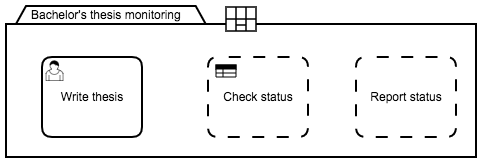
\includegraphics[width=0.8\textwidth]{../figures/chapter_combinations/CMMN_thesis_decision_task.png} 
\caption{CMMN case with a decision task linking to a DMN decision table.}
\label{fig:CMMN_with_Decision_task}
\end{figure}
%-------------------------------------------------------------------------

Figure \ref{fig:CMMN_with_Decision_task} shows a simple case with a discretionary decision task modeled. The scenario deals with a student who has to write his bachelor's thesis (see Human Task) and is monitored by his supervisor. The decision task incorporates the decision logic and links to a DMN table. When the case worker, presumably the student, needs to report the thesis' status to his supervisor, he checks the decision table that aggregates the information and outputs the status. In this example, the worker simply enters the amount of written pages and a comment, for instance \textit{on track} or \textit{far behind}, is presented. The student sends this result afterwards to his supervisor.\\ 
This brief example use case demonstrated an automated decision making in an environment where the focus lies on human behavior and human reacting. As DMN serves not only as a \texttt{decision-making} notation, but also as a possibility to process data and generate an output in a fast and flexible way, it helps knowledge workers to react to data-intensive tasks and to plan following discretionary steps. 

%At this point we can conclude: there is nothing mentioned in the specification to link DMN processes. Examining the Signavio modeler (version 10.5.0, September 2016), it apparently is possible to link DMN models with a process with task. The camunda modeler (version 1.3.0, September 2016) is also able make a reference to a DMN process. However, there are inconsistencies. Listing \ref{xml:signavio} represents a snippet of XML code that is generated with signavio modeler. The snippet focuses on the process task with the linked DMN model. However, there is no reference to the linked model, which is either due to the current beta status or an incompatibility. Listing \ref{xml:camunda} shows another XML file of a CMMN model with the exact same process task and a DMN model linked. This time modeled in with the Camunda modeler. 
%
%\begin{lstlisting}[caption=XML file of a process task modeled with signavio modeler, label=xml:signavio]
%	<rdf:Description rdf:about="#sid-0083FC24-78CC-4C77-B527-5BC8B8956439">
%		<type xmlns="http://oryx-editor.org/">ProcessTask</type>
%		<bounds xmlns="http://oryx-editor.org/">261.4288403563878,97.08155333081379,
%		162.28652106916334,17.24465999244137</bounds>
%		<discretionary xmlns="http://oryx-editor.org/">false</discretionary>
%		<entry xmlns="http://oryx-editor.org/">/model/5a1ebf9abcce4bbdbd04a3b9d1652d6a</entry>
%		<bgcolor xmlns="http://oryx-editor.org/">#FFFFCC</bgcolor>
%		<name xmlns="http://oryx-editor.org/">test
%		</name>
%		<description xmlns="http://oryx-editor.org/"/>
%		<type xmlns="http://oryx-editor.org/">http://signavio.com/stencilsets/cmmn-1.0#Task</type>
%		<repetition xmlns="http://oryx-editor.org/">false</repetition>
%		<manualactivation xmlns="http://oryx-editor.org/">false</manualactivation>
%		<required xmlns="http://oryx-editor.org/">false</required>
%		<bordercolor xmlns="http://oryx-editor.org/">#000000</bordercolor>
%		<docker xmlns="http://oryx-editor.org/"> # </docker>
%		<parent xmlns="http://raziel.org/" rdf:resource="#sid-F6DDC76E-A454-4C2F-A7D1-4121A78A527F"/>
%	</rdf:Description>
%\end{lstlisting} 
%
%\begin{lstlisting}[caption=A Process Task modeled with camunda modeler, label=xml:camunda]
%  <cmmn:case id="Case_1">
%    <cmmn:casePlanModel id="CasePlanModel_1" name="A CasePlanModel">
%      <cmmn:planItem id="PlanItem_1" definitionRef="ProcessTask_1nzv0h6" />
%      <cmmn:processTask id="ProcessTask_1nzv0h6" name="TASK" processRef="DMN_MODEL.dmn" /> |\label{line:processRef}|
%    </cmmn:casePlanModel>
%  </cmmn:case>
%\end{lstlisting}
%
%Here, in line \ref{line:processRef} of Listing \ref{xml:camunda}, the reference to the DMN model is documented, whereas Listing \ref{xml:signavio} does not provide any reference to the according attribute, although the process is visually linked in the modeler. Unfortunately, it wasn't possible to execute neither the camunda version nor the signavio one. The latter is still in beta phase and the former one cannot be executed without any licensing. We asked for an academic license but could not acquire one. \\
%Reviewing the results, integrating DMN in CMMN is not namely intended, but it seems possible. The Camunda example showed a reference that could be set to a DMN model, which was also possible with the Signavio modeler. However, the Signavio XML file did not show the \texttt{processRef} attribute which, in fact, is the link to external processes. \\
%Integrating CMMN in DMN, on the other hand, is impossible as DMN has not interface to external processes such as BPMN Call Activities or CMMN Process Tasks. 
